% =========================================================
%  Chapter 9 — Laser Diode Dynamics, Modulation, and
%              Single-Frequency Operation
%  Source: Dr. George's Lectures (Lecture 5)
%  Style: student-voice notes matching the personal style guide
% =========================================================

% ------------------------------------------------------------------
\section{Beyond the DC Picture}
% ------------------------------------------------------------------

The previous chapter derived the complete static behaviour of the laser diode: threshold carrier density, carrier clamping above threshold, and the linear P--I characteristic. All of this assumed that the device had settled to steady state and that current, carrier density, and photon density were all constant. In a real communications system, the drive current is modulated at gigabit-per-second rates, and none of those quantities is ever truly constant. The laser must respond faithfully to every current fluctuation, and the rate at which it can do so is finite.

This chapter reveals the dynamic behaviour that is completely hidden in the DC analysis. We start from the same coupled carrier-photon rate equations and solve them for a \emph{time-varying} drive, discovering a rich resonance phenomenon — the relaxation oscillation — that fundamentally limits modulation bandwidth. We then tackle large-signal switching and the turn-on delay, and finally examine how to eliminate the multi-mode problem of the Fabry-Pérot cavity by using wavelength-selective feedback in the DFB and DBR laser architectures.

% ------------------------------------------------------------------
\section{The Coupled Rate Equations}
% ------------------------------------------------------------------

The full dynamical system governing the laser diode couples two state variables — carrier density $N(t)$ and photon density $S(t)$ — through two simultaneous first-order ODEs:
\begin{keyresult}
    \begin{gather}
        \frac{dN}{dt} = \frac{J}{ed} - \frac{N}{\tau} - \Gamma B(N - N_\text{tr})S \\[6pt]
        \frac{dS}{dt} = \Gamma B(N - N_\text{tr})S - \frac{S}{\tau_{ph}} + \beta\,\frac{N}{\tau_r}
    \end{gather}
\end{keyresult}

The physical role of each term has been established in the previous chapter. The new element here is that we are keeping both equations simultaneously and allowing both $N$ and $S$ to vary in time. The coupling is through the stimulated emission term $\Gamma B(N - N_\text{tr})S$: it appears as a \emph{loss} in the carrier equation (stimulated emission depletes carriers) and as a \emph{gain} in the photon equation (the same stimulated process generates photons).

% ------------------------------------------------------------------
\section{Small-Signal Modulation Analysis}
% ------------------------------------------------------------------

\subsection{Linearisation Around the Bias Point}

For small-signal modulation, we bias the laser above threshold at a steady operating point $(N_0, S_0)$ and superimpose a small sinusoidal perturbation at modulation frequency $\omega_m$:
\begin{equation*}
    J(t) = J_0 + J_m e^{j\omega_m t}, \qquad N(t) = N_0 + N_m e^{j\omega_m t}, \qquad S(t) = S_0 + S_m e^{j\omega_m t}
\end{equation*}
where $J_m \ll J_0$, $N_m \ll N_0$, and $S_m \ll S_0$ represent the small-signal AC amplitudes. Since the laser is biased above threshold, the steady-state carrier density is clamped at the threshold value, so $N_0 = N_\text{th}$.

Substituting these perturbed quantities into the coupled rate equations yields:
\begin{align*}
    \frac{d(N_0 + N_m e^{j\omega_m t})}{dt} &= \frac{J_0 + J_m e^{j\omega_m t}}{ed} - \frac{N_0 + N_m e^{j\omega_m t}}{\tau} - \Gamma B\left(N_0 + N_m e^{j\omega_m t} - N_\text{tr}\right)\left(S_0 + S_m e^{j\omega_m t}\right) \\[6pt]
    \frac{d(S_0 + S_m e^{j\omega_m t})}{dt} &= \Gamma B\left(N_0 + N_m e^{j\omega_m t} - N_\text{tr}\right)\left(S_0 + S_m e^{j\omega_m t}\right) - \frac{S_0 + S_m e^{j\omega_m t}}{\tau_{ph}} + \beta\frac{N_0 + N_m e^{j\omega_m t}}{\tau_r}
\end{align*}

To linearise this system, we expand the terms and make the following physical simplifications:
\begin{enumerate}
    \item We expand the stimulated emission term, noting that:
    \begin{align*}
        \Gamma B(N_0 + N_m e^{j\omega_m t} - N_\text{tr})(S_0 + S_m e^{j\omega_m t}) = \Gamma B(N_0 - N_\text{tr})S_0 &+ \Gamma B S_0 N_m e^{j\omega_m t} \\
        &+ \Gamma B(N_0 - N_\text{tr})S_m e^{j\omega_m t} + \Gamma B N_m S_m e^{2j\omega_m t}
    \end{align*}
    \item We drop the second-order small AC product term, $\Gamma B N_m S_m e^{2j\omega_m t} \approx 0$.
    \item We neglect the contribution of spontaneous emission to the AC dynamics above threshold, setting $\beta \frac{N_m e^{j\omega_m t}}{\tau_r} \approx 0$ (since the spontaneous emission factor $\beta \approx 10^{-4}$ is extremely small and stimulated processes dominate the AC response).
\end{enumerate}

Applying these approximations and performing the differentiation on the left-hand side ($d/dt \to j\omega_m$) gives:
\begin{align*}
    j\omega_m N_m e^{j\omega_m t} &= \left[ \frac{J_0}{ed} - \frac{N_0}{\tau} - \Gamma B(N_0 - N_\text{tr})S_0 \right] + \left[ \frac{J_m}{ed} - \frac{N_m}{\tau} - \Gamma B S_0 N_m - \Gamma B(N_0 - N_\text{tr})S_m \right] e^{j\omega_m t} \\[6pt]
    j\omega_m S_m e^{j\omega_m t} &= \left[ \Gamma B(N_0 - N_\text{tr})S_0 - \frac{S_0}{\tau_{ph}} + \beta\frac{N_0}{\tau_r} \right] + \left[ \Gamma B S_0 N_m + \left( \Gamma B(N_0 - N_\text{tr}) - \frac{1}{\tau_{ph}} \right) S_m \right] e^{j\omega_m t}
\end{align*}

By definition, the DC terms inside the first brackets on the right-hand sides must balance the steady-state (zero-derivative) rate equations:
\begin{align*}
    0 &= \frac{J_0}{ed} - \frac{N_0}{\tau} - \Gamma B(N_0 - N_\text{tr})S_0 \\[6pt]
    0 &= \Gamma B(N_0 - N_\text{tr})S_0 - \frac{S_0}{\tau_{ph}} + \beta\frac{N_0}{\tau_r}
\end{align*}
Therefore, the DC terms cancel identically. Furthermore, since the laser is biased above threshold ($N_0 = N_\text{th}$), the gain clamps to the cavity loss:
\begin{equation*}
    \Gamma B(N_\text{th} - N_\text{tr}) = \frac{1}{\tau_{ph}}
\end{equation*}
This causes the $\left(\Gamma B(N_0 - N_\text{tr}) - 1/\tau_{ph}\right) S_m$ term in the AC photon equation to vanish. Cancelling the common factor $e^{j\omega_m t}$ leaves a clean linear system for the AC amplitudes:
\begin{equation*}
    j\omega_m N_m = \frac{J_m}{ed} - \left(\frac{1}{\tau} + \Gamma B S_0\right)N_m - \Gamma B(N_\text{th} - N_\text{tr})S_m
\end{equation*}
\begin{equation*}
    j\omega_m S_m = \Gamma B S_0\,N_m
\end{equation*}

The second equation expresses a simple fact: photon density fluctuations are driven purely by carrier density fluctuations through the stimulated emission term $\Gamma B S_0$ (the steady-state photon density acts as the amplifier for carrier perturbations).

\subsection{The Modulation Transfer Function}

We eliminate $N_m$ between the two equations to get the optical response $S_m$ as a function of the current modulation $J_m$. Using the threshold relation $\Gamma B(N_\text{th} - N_\text{tr}) = 1/\tau_{ph}$ to simplify, and defining a convenient stimulated lifetime:
\begin{keyresult}
    \begin{equation}
        \frac{1}{\tau_{st}} \equiv \Gamma B S_0
    \end{equation}
\end{keyresult}

The stimulated lifetime $\tau_{st}$ is the average time a carrier spends before being consumed by stimulated emission into the photon mode. Above threshold with strong photon density $S_0$, this can be much shorter than the spontaneous lifetime $\tau$. We now eliminate $N_m$ explicitly. From the photon AC equation, we isolate $N_m$:
\begin{equation*}
    N_m = \frac{j\omega_m S_m}{\Gamma B S_0} = j\omega_m\tau_{st}\,S_m
\end{equation*}
Substituting this expression for $N_m$ into the carrier AC equation, and replacing $\Gamma B(N_\text{th} - N_\text{tr})$ with $1/\tau_{ph}$:
\begin{equation*}
    j\omega_m(j\omega_m\tau_{st}\,S_m) = \frac{J_m}{ed} - \left(\frac{1}{\tau} + \frac{1}{\tau_{st}}\right)(j\omega_m\tau_{st}\,S_m) - \frac{S_m}{\tau_{ph}}
\end{equation*}
Using $j^2 = -1$, this simplifies to:
\begin{equation*}
    -\omega_m^2\tau_{st}\,S_m = \frac{J_m}{ed} - j\omega_m\tau_{st}\left(\frac{1}{\tau} + \frac{1}{\tau_{st}}\right)S_m - \frac{S_m}{\tau_{ph}}
\end{equation*}
To solve for $S_m$, we collect all terms containing $S_m$ on the left-hand side:
\begin{equation*}
    -\omega_m^2\tau_{st}\,S_m + j\omega_m\tau_{st}\left(\frac{1}{\tau} + \frac{1}{\tau_{st}}\right)S_m + \frac{S_m}{\tau_{ph}} = \frac{J_m}{ed}
\end{equation*}
Dividing both sides by $\tau_{st}$ to isolate the second-order frequency term:
\begin{equation*}
    S_m\left[ -\omega_m^2 + j\omega_m\left(\frac{1}{\tau} + \frac{1}{\tau_{st}}\right) + \frac{1}{\tau_{st}\,\tau_{ph}} \right] = \frac{J_m}{ed\,\tau_{st}}
\end{equation*}
We now define the system parameters: the relaxation oscillation frequency $\omega_r^2 = 1/(\tau_{st}\tau_{ph})$ and the damping factor $\xi = 1/\tau + 1/\tau_{st}$. Substituting these in:
\begin{equation*}
    S_m\left[ \omega_r^2 + j\omega_m\xi - \omega_m^2 \right] = \frac{J_m}{ed\,\tau_{st}}
\end{equation*}
Dividing both sides by $\omega_r^2$:
\begin{equation*}
    S_m\left[ 1 + j\frac{\xi\omega_m}{\omega_r^2} - \left(\frac{\omega_m}{\omega_r}\right)^2 \right] = \frac{J_m}{ed\,\tau_{st}\omega_r^2}
\end{equation*}
Since $\omega_r^2 = 1/(\tau_{st}\tau_{ph})$, the numerator on the right becomes:
\begin{equation*}
    \frac{1}{ed\,\tau_{st}\omega_r^2} = \frac{\tau_{st}\tau_{ph}}{ed\,\tau_{st}} = \frac{\tau_{ph}}{ed} = H_0
\end{equation*}
This yields the standard second-order transfer function $H(j\omega_m)$:
\begin{keyresult}
    \begin{equation}
        H(j\omega_m) = \frac{S_m}{J_m} = \frac{H_0}{1 + j\,\dfrac{\xi\,\omega_m}{\omega_r^2} - \left(\dfrac{\omega_m}{\omega_r}\right)^2}, \qquad H_0 = \frac{\tau_{ph}}{ed}
    \end{equation}
\end{keyresult}
where the two key system parameters are:
\begin{keyresult}
    \begin{gather}
        \omega_r^2 = \frac{\Gamma B S_0}{\tau_{ph}} = \frac{1}{\tau_{st}\,\tau_{ph}} \\[6pt]
        \xi = \frac{1}{\tau} + \Gamma B S_0 = \frac{1}{\tau} + \frac{1}{\tau_{st}}
    \end{gather}
\end{keyresult}

\begin{figure}[H]
    \centering
    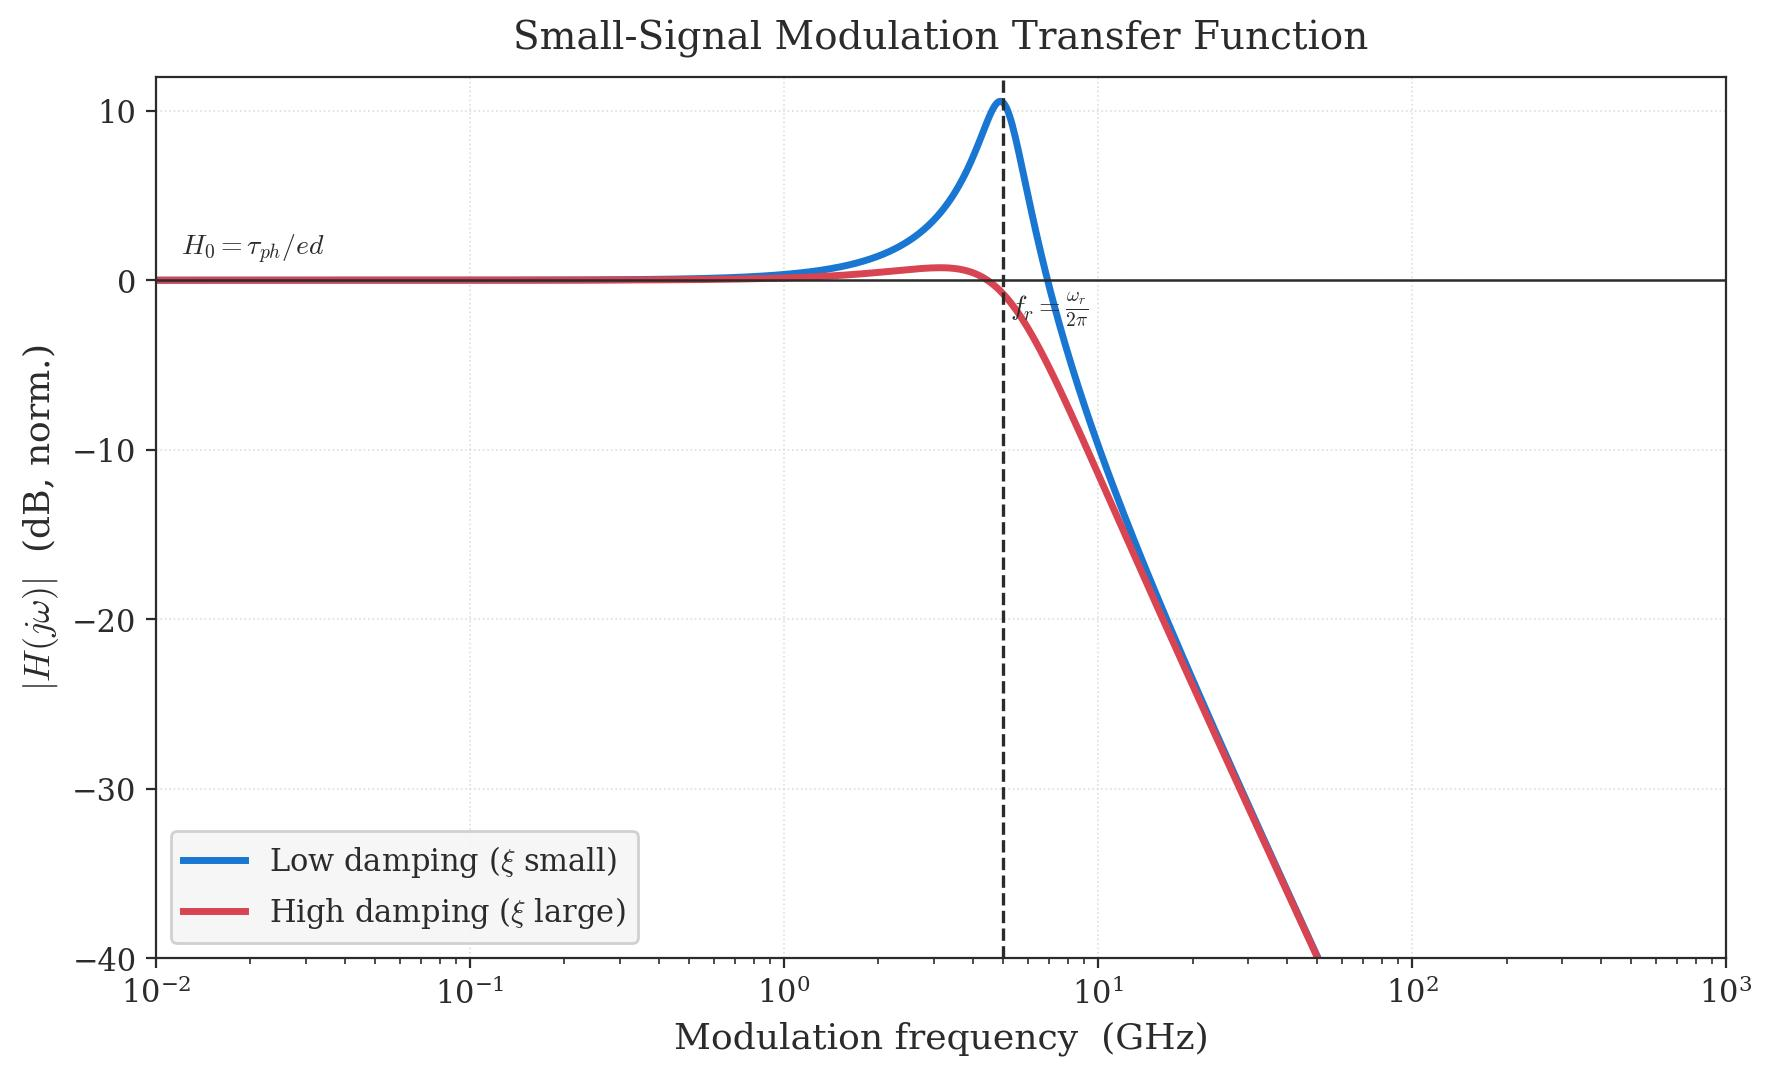
\includegraphics[width=0.6\textwidth]{Figures/Chapter 9/modulation_transfer_function.jpg}
    \caption{Small-Signal Modulation Transfer Function}
    \label{fig:modulation_transfer_function}
\end{figure}

$\omega_r$ is the \textbf{relaxation oscillation frequency} — the natural resonance frequency of the coupled carrier-photon system. $\xi$ is the \textbf{damping factor} — it determines how quickly oscillations decay after a perturbation. $H_0 = \tau_{ph}/ed$ is the low-frequency (DC) modulation efficiency.

\begin{figure}[H]
    \centering
    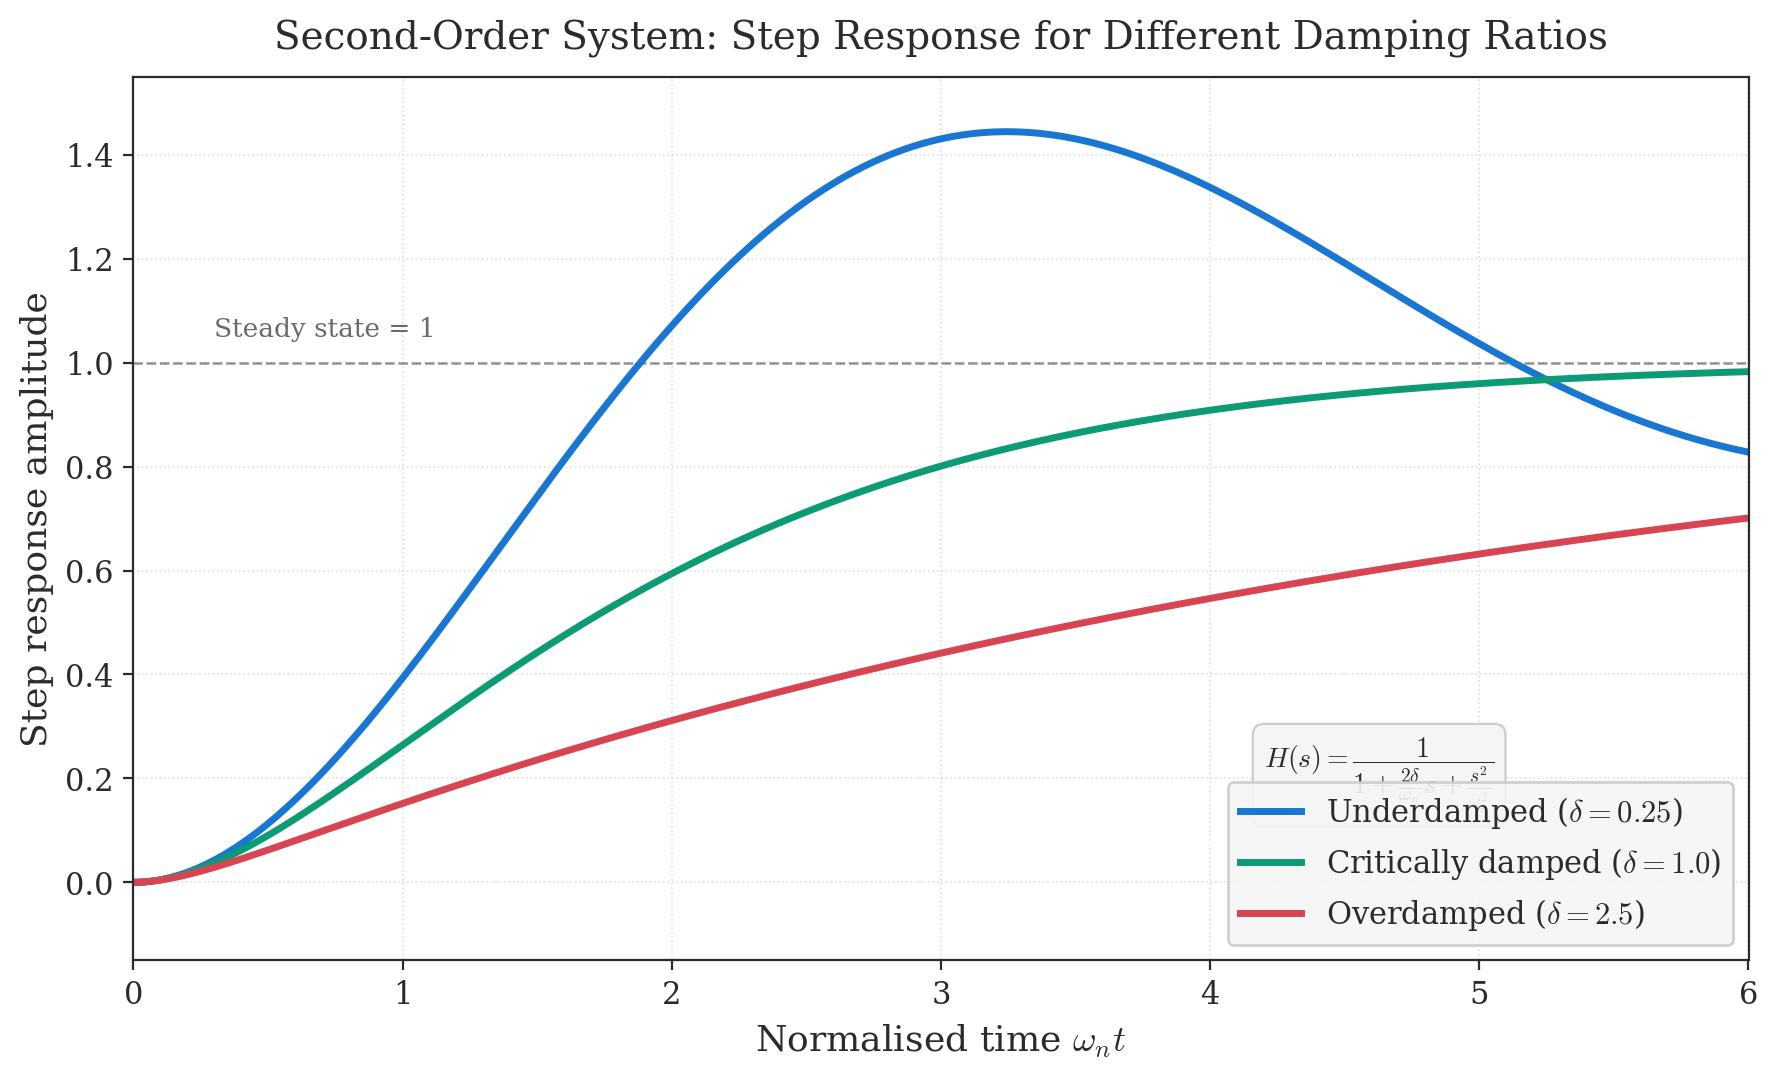
\includegraphics[width=0.6\textwidth]{Figures/Chapter 9/second_order_damping.jpg}
    \caption{Generic Second-Order Response and Damping Cases}
    \label{fig:second_order_damping}
\end{figure}

\subsection{Physical Interpretation of the Resonance}

The second-order denominator reveals a resonance: at $\omega_m = \omega_r$, the response peaks above its DC value if the damping is light enough. The physics behind this resonance is a feedback loop between the two rate equations:

A current step injects extra carriers. The extra carriers increase the gain, which causes the photon density to rise. The rising photon density depletes carriers faster via stimulated emission, so the carrier density overshoots downward. With fewer carriers, the gain drops, and the photon density falls. This reduction in photon density releases the stimulated emission pressure, allowing the carrier density to recover upward again. The system oscillates back and forth — this is the relaxation oscillation.

The frequency of this oscillation scales as $\omega_r \propto \sqrt{S_0/\tau_{ph}}$: a higher steady-state photon density (stronger bias above threshold) and a shorter photon lifetime (lossier cavity) both push the resonance to higher frequencies.

\subsection{Bias-Dependence: Scaling with Normalised Current}

Expressing results in terms of the normalised current $m = I/I_\text{th}$ and using the above-threshold approximation $(m-1)\tau_{ph}/\tau \approx \tau/\tau_{st}$ gives compact scaling laws:
\begin{equation*}
    \tau_{st} = \frac{\tau}{m-1}, \qquad \omega_r^2 = \frac{m-1}{\tau_{ph}\,\tau}, \qquad \xi = \frac{m}{\tau}
\end{equation*}

These reveal how the three modulation parameters evolve as we increase the bias:
\begin{itemize}
    \item $\omega_r$ grows as $\sqrt{m-1}$: biasing harder above threshold pushes the relaxation resonance to higher frequencies, increasing the potential modulation bandwidth.
    \item $\xi$ grows linearly with $m$: heavier bias also increases the damping, which suppresses the resonance peak and reduces ringing.
    \item At practical bias levels, the bandwidth is limited to a few times $\omega_r/(2\pi)$ — typically in the range of 10--30\,GHz for state-of-the-art edge-emitting laser diodes.
\end{itemize}

\begin{figure}[H]
    \centering
    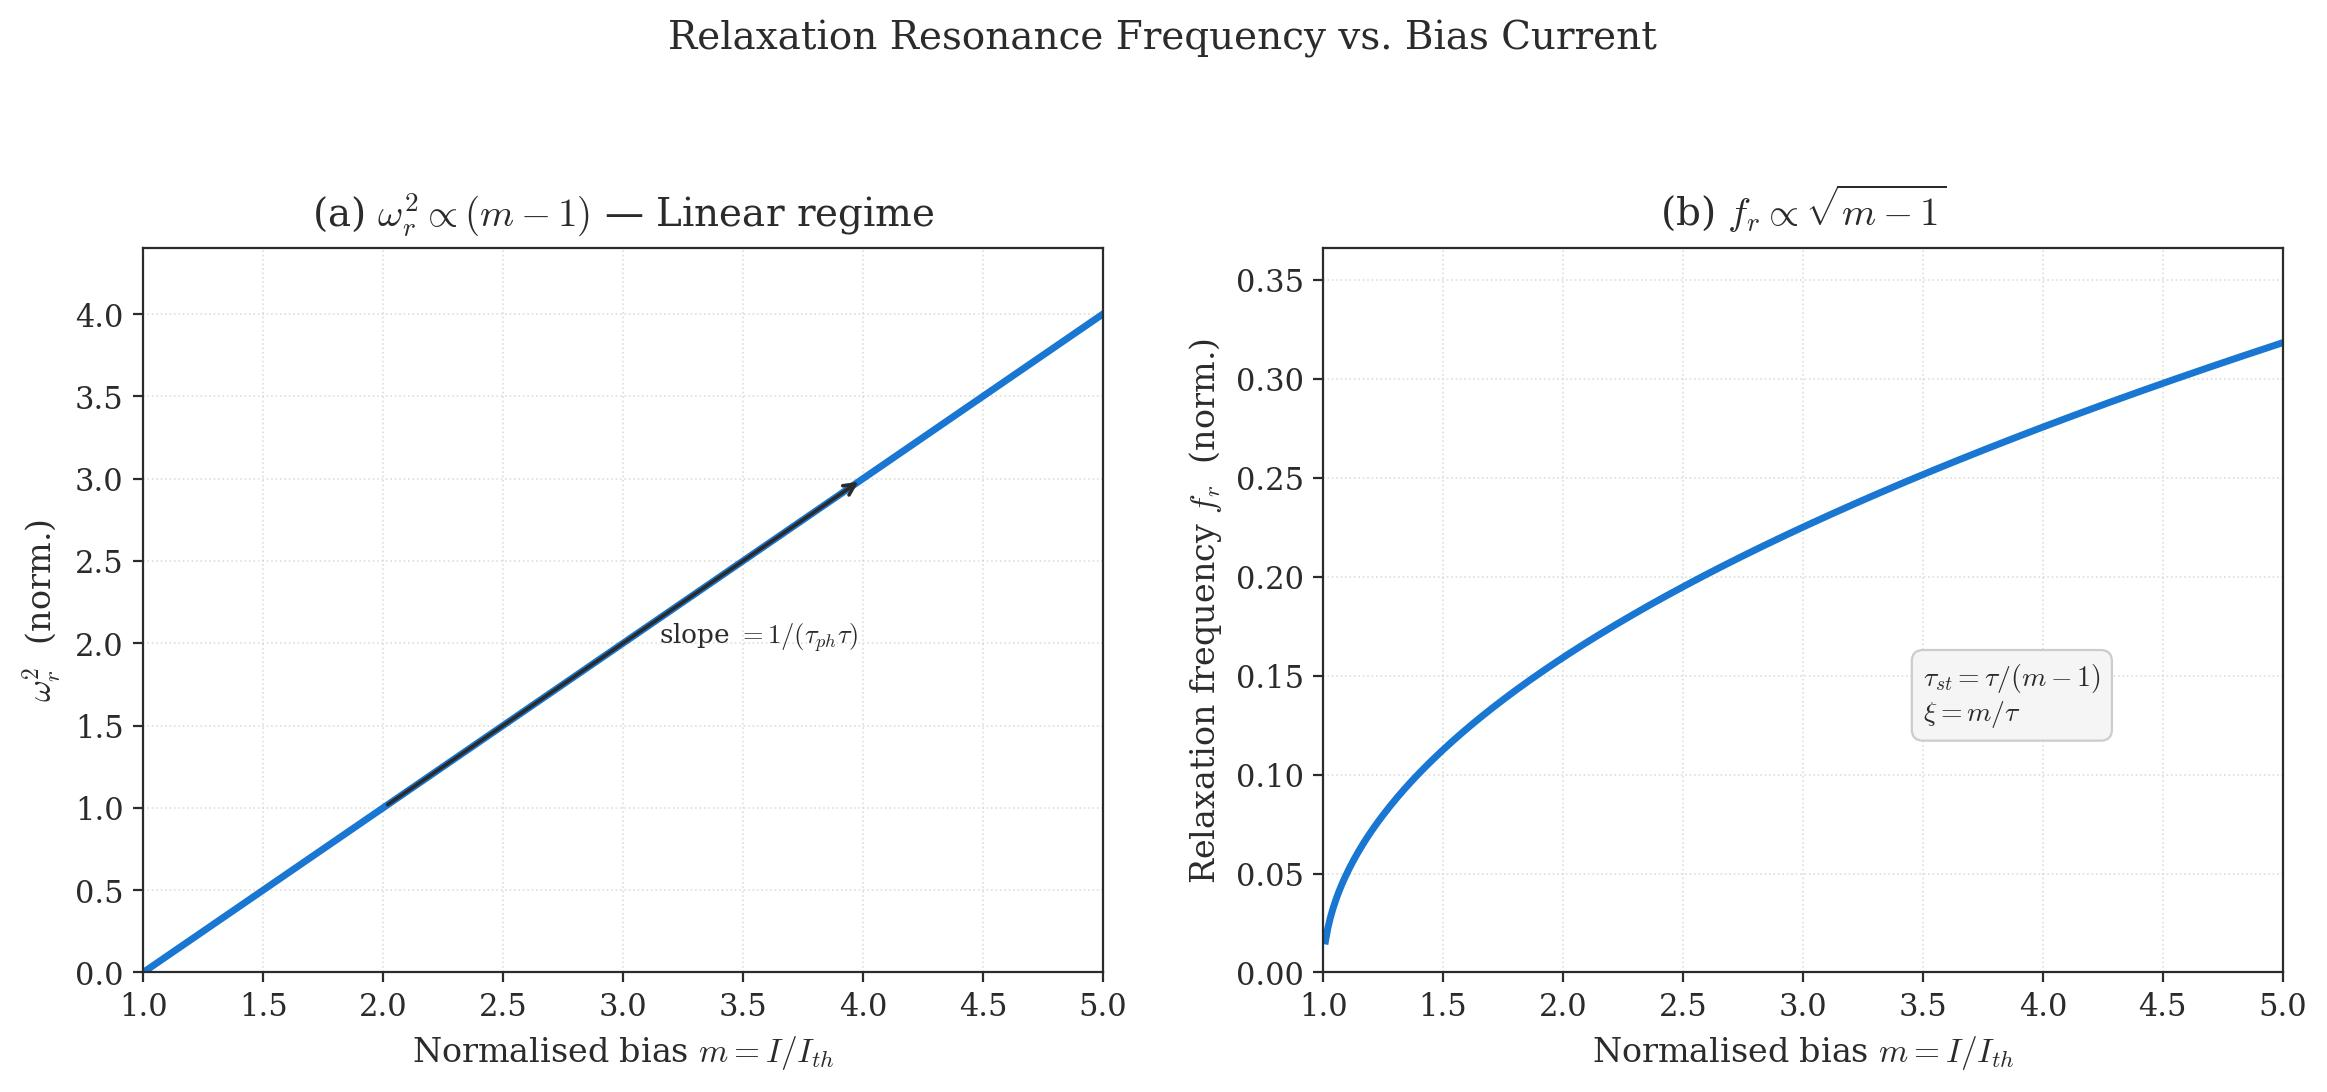
\includegraphics[width=0.6\textwidth]{Figures/Chapter 9/relaxation_freq_vs_bias.jpg}
    \caption{Relaxation Frequency Versus Bias Current}
    \label{fig:relaxation_freq_vs_bias}
\end{figure}

% ------------------------------------------------------------------
\section{Large-Signal Modulation: Turn-On Delay}
% ------------------------------------------------------------------

\subsection{Charging the Carrier Reservoir}

The small-signal analysis assumed infinitesimally small current perturbations. For digital data links, the laser is switched hard from a low current $I_1$ (near or below threshold) to a high current $I_2$ (well above threshold) to encode a "1" bit. During the initial charging phase, the photon density is still negligible — stimulated emission has not yet ignited — and the carrier rate equation simplifies to a single exponential charging equation:
\begin{equation*}
    N(t) = N_1 + (N_2 - N_1)\left(1 - e^{-t/\tau}\right)
\end{equation*}
where $N_1 = J_1\tau/(ed)$ and $N_2 = J_2\tau/(ed)$ are the steady-state carrier densities corresponding to the two current levels.

The laser does not begin lasing until $N(t)$ reaches the threshold density $N_\text{th}$. The time required to reach $N_\text{th}$ is the \textbf{turn-on delay} $t_d$. To solve for $t_d$, we set $N(t_d) = N_\text{th}$:
\begin{equation*}
    N_\text{th} = N_1 + (N_2 - N_1)\left(1 - e^{-t_d/\tau}\right)
\end{equation*}
Rearranging to isolate the exponential term:
\begin{equation*}
    (N_2 - N_1)e^{-t_d/\tau} = N_2 - N_\text{th} \implies e^{-t_d/\tau} = \frac{N_2 - N_\text{th}}{N_2 - N_1}
\end{equation*}
Taking the natural logarithm of both sides:
\begin{equation*}
    -\frac{t_d}{\tau} = \ln\!\left(\frac{N_2 - N_\text{th}}{N_2 - N_1}\right) \implies t_d = \tau \ln\!\left(\frac{N_2 - N_1}{N_2 - N_\text{th}}\right)
\end{equation*}
Since the carrier densities correspond to steady-state sub-threshold relationships, they are directly proportional to their drive current densities ($N_i = J_i\tau/ed$). Substituting $N_1 = J_1\tau/(ed)$, $N_2 = J_2\tau/(ed)$, and $N_\text{th} = J_\text{th}\tau/(ed)$, the common prefactor $\tau/(ed)$ cancels from the numerator and denominator:
\begin{keyresult}
    \begin{equation}
        t_d = \tau\ln\!\left(\frac{J_2 - J_1}{J_2 - J_\text{th}}\right)
    \end{equation}
\end{keyresult}

\begin{figure}[H]
    \centering
    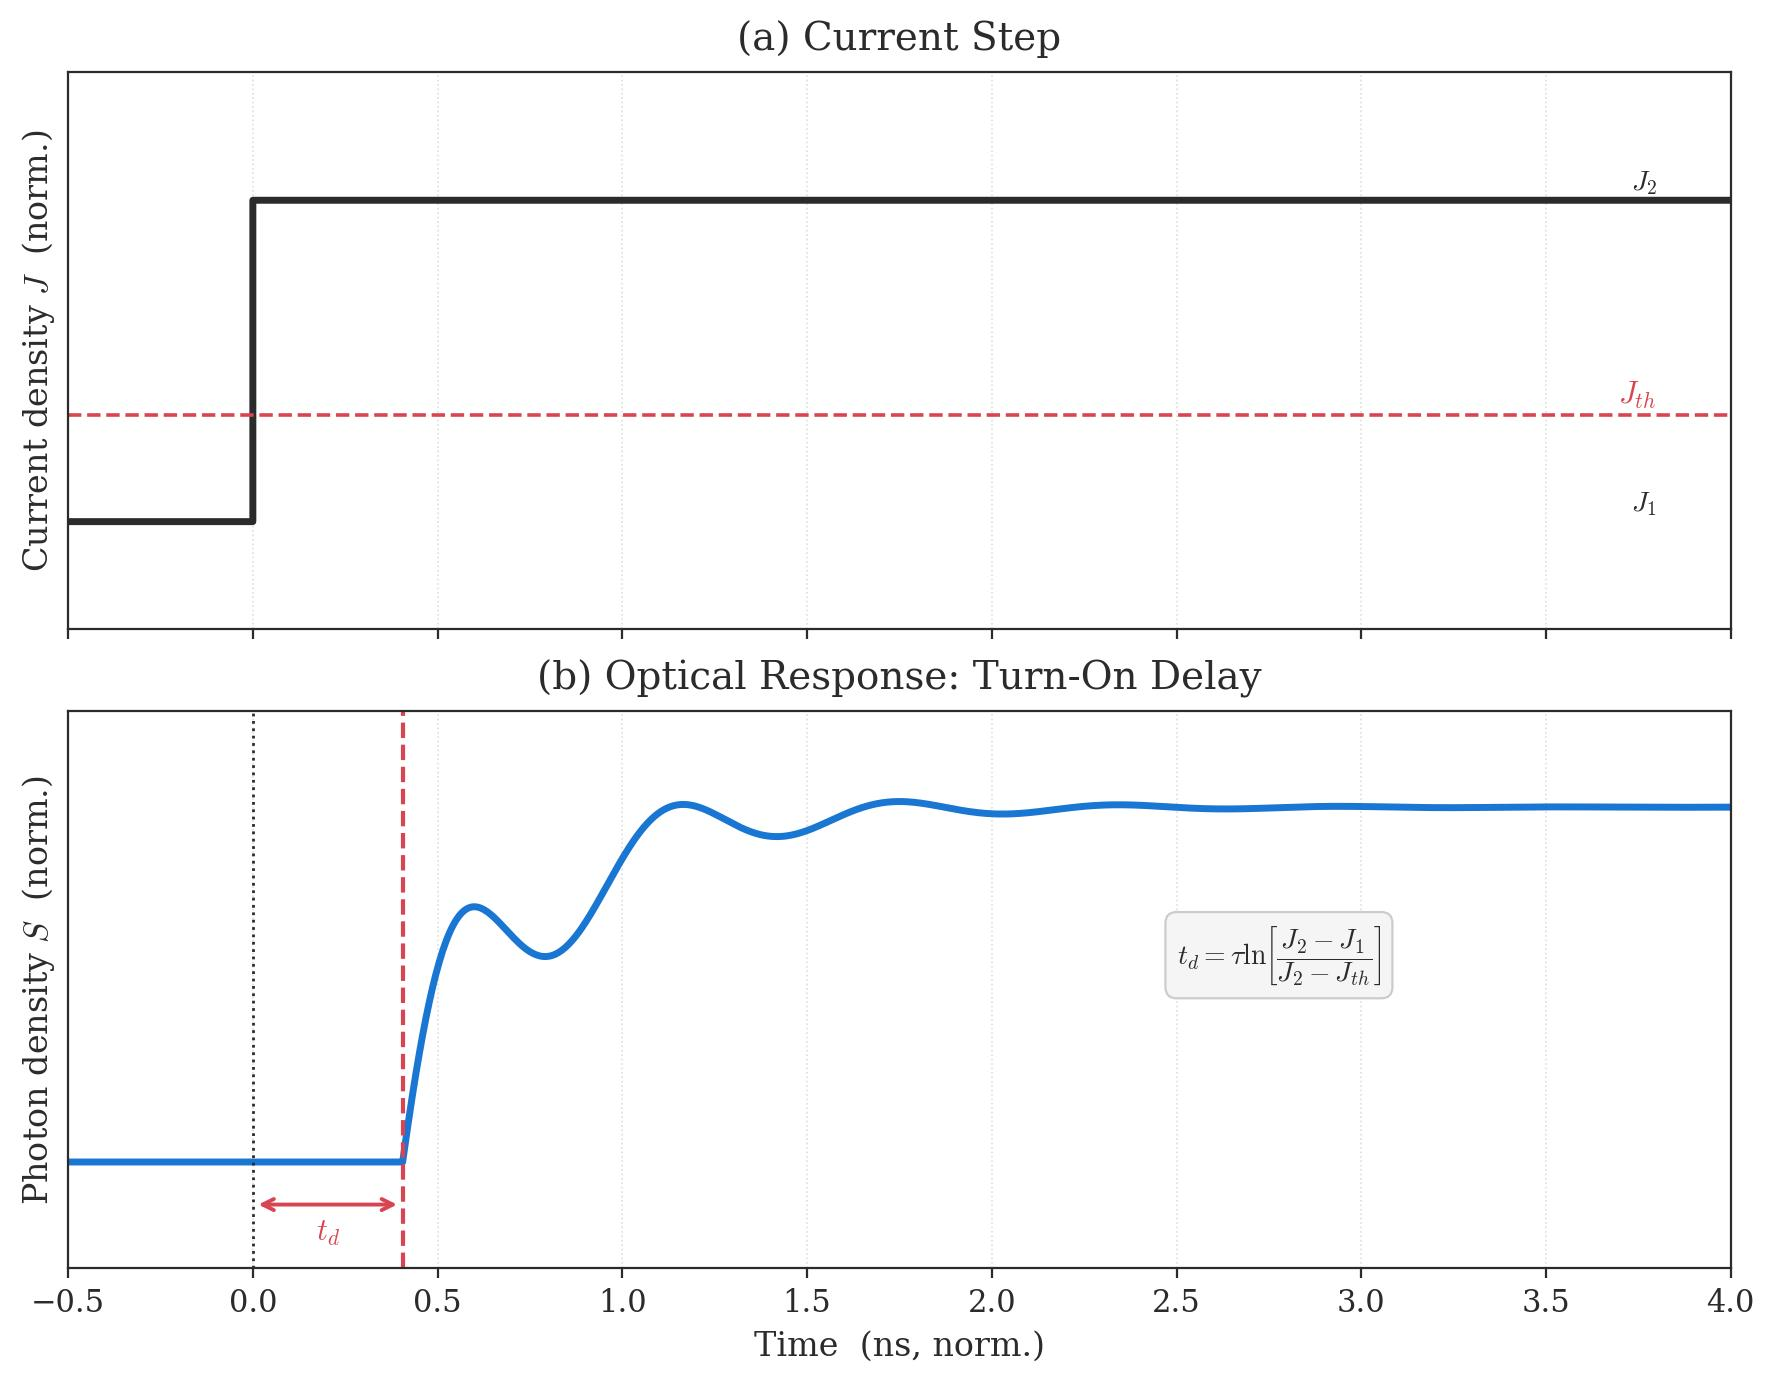
\includegraphics[width=0.7\textwidth]{Figures/Chapter 9/turnon_delay.jpg}
    \caption{Turn-On Delay After a Current Step}
    \label{fig:turnon_delay}
\end{figure}

This formula encodes two familiar engineering strategies:

A \emph{larger current step} (higher $J_2$) makes the ratio $(J_2 - J_1)/(J_2 - J_\text{th})$ approach unity, so $t_d \to 0$. Driving with as much current as the device can tolerate minimises turn-on delay.

\emph{Pre-biasing} the laser at $J_1$ close to $J_\text{th}$ makes $N_1$ close to $N_\text{th}$, so the carrier density needs only a tiny additional push to reach threshold. Even a small residual bias on the "0" level dramatically reduces $t_d$ at the cost of slightly reduced extinction ratio.

\subsection{Relaxation Oscillations After Turn-On}

Once the carrier density crosses $N_\text{th}$, stimulated emission ignites and the photon density rises rapidly. But the coupled system does not settle immediately — the same resonance mechanism responsible for the small-signal peak drives transient oscillations. We linearise the rate equations for time-domain deviations $\Delta N(t) = N(t) - N_\text{th}$ and $\Delta S(t) = S(t) - S_0$ around the final above-threshold steady-state point $(N_\text{th}, S_0)$:
\begin{align*}
    \frac{d(N_\text{th} + \Delta N)}{dt} &= \frac{J_2}{ed} - \frac{N_\text{th} + \Delta N}{\tau} - \Gamma B(N_\text{th} + \Delta N - N_\text{tr})(S_0 + \Delta S) \\[6pt]
    \frac{d(S_0 + \Delta S)}{dt} &= \Gamma B(N_\text{th} + \Delta N - N_\text{tr})(S_0 + \Delta S) - \frac{S_0 + \Delta S}{\tau_{ph}} + \beta\frac{N_\text{th} + \Delta N}{\tau_r}
\end{align*}

We subtract the DC steady-state relations (with $J = J_2$ and spontaneous emission neglected for the dynamic deviation), drop the second-order perturbation product $\Delta N \Delta S \approx 0$, and apply the gain clamping condition $\Gamma B(N_\text{th} - N_\text{tr}) = 1/\tau_{ph}$. This yields the linearized first-order system:
\begin{align*}
    \frac{d\,\Delta N}{dt} &= -\left(\frac{1}{\tau} + \Gamma B S_0\right)\Delta N - \Gamma B(N_\text{th} - N_\text{tr})\,\Delta S = -\xi\,\Delta N - \frac{\Delta S}{\tau_{ph}} \\[6pt]
    \frac{d\,\Delta S}{dt} &= \Gamma B S_0\,\Delta N = \frac{\Delta N}{\tau_{st}}
\end{align*}
where we have used the definitions $\xi = 1/\tau + \Gamma B S_0$ and $\tau_{st} = 1/(\Gamma B S_0)$.

To combine these into a single equation, we differentiate the carrier equation with respect to time:
\begin{equation*}
    \frac{d^2\Delta N}{dt^2} = -\xi\,\frac{d\,\Delta N}{dt} - \frac{1}{\tau_{ph}}\frac{d\,\Delta S}{dt}
\end{equation*}
Substituting the derivative of the photon density $\frac{d\,\Delta S}{dt} = \Gamma B S_0\,\Delta N$ into the equation:
\begin{equation*}
    \frac{d^2\Delta N}{dt^2} = -\xi\,\frac{d\,\Delta N}{dt} - \frac{\Gamma B S_0}{\tau_{ph}}\,\Delta N
\end{equation*}
Since $\omega_r^2 = \frac{\Gamma B S_0}{\tau_{ph}}$, this rearranges into the classic second-order damped harmonic oscillator ODE:
\begin{keyresult}
    \begin{equation}
        \frac{d^2\Delta N}{dt^2} + \xi\,\frac{d\Delta N}{dt} + \omega_r^2\,\Delta N = 0
    \end{equation}
\end{keyresult}

We solve this using the characteristic equation $s^2 + \xi s + \omega_r^2 = 0$. The roots are:
\begin{equation*}
    s_{1,2} = -\frac{\xi}{2} \pm j\sqrt{\omega_r^2 - \left(\frac{\xi}{2}\right)^2} = -\frac{\xi}{2} \pm j\Omega
\end{equation*}
where $\Omega \equiv \sqrt{\omega_r^2 - (\xi/2)^2}$ is the damped oscillation frequency. For the underdamped case ($\xi < 2\omega_r$), the carrier density solution is a decaying sinusoid:
\begin{keyresult}
    \begin{equation}
        \Delta N(t) = D\,e^{-(\xi/2) t}\sin(\Omega\,t)
    \end{equation}
\end{keyresult}
where $D$ is a constant determined by the initial conditions of the current step. 

To find the corresponding photon density deviation $\Delta S(t)$, we integrate the linearized photon equation:
\begin{equation*}
    \Delta S(t) = \Gamma B S_0 \int \Delta N(t)\,dt = \Gamma B S_0 D \int e^{-(\xi/2) t}\sin(\Omega\,t)\,dt
\end{equation*}
Using the standard integration identity $\int e^{-at} \sin(\Omega t)\,dt = -\frac{e^{-at}}{a^2+\Omega^2}(a\sin(\Omega t) + \Omega\cos(\Omega t))$ with $a = \xi/2$:
\begin{equation*}
    \Delta S(t) = -\Gamma B S_0 D \frac{e^{-(\xi/2) t}}{(\xi/2)^2 + \Omega^2} \left[ \frac{\xi}{2}\sin(\Omega\,t) + \Omega\cos(\Omega\,t) \right]
\end{equation*}
Since $(\xi/2)^2 + \Omega^2 = \omega_r^2$ and we are in the typical light-damping limit where the decay rate is much slower than the oscillation frequency ($\xi/2 \ll \Omega$), the sine term inside the brackets is negligible. Using this approximation:
\begin{equation*}
    \Delta S(t) \approx -\frac{\Gamma B S_0 D \Omega}{\omega_r^2} e^{-(\xi/2) t}\cos(\Omega\,t)
\end{equation*}
Using the identity $\omega_r^2 = \frac{\Gamma B S_0}{\tau_{ph}} \implies \frac{\Gamma B S_0}{\omega_r^2} = \tau_{ph}$, and substituting $\omega_r \approx \Omega$ under light damping:
\begin{keyresult}
    \begin{equation}
        \Delta S(t) \approx -\frac{\Gamma B S_0}{\Omega}\,D\,e^{-(\xi/2) t}\cos(\Omega\,t) \approx -\tau_{ph}\Omega D\,e^{-(\xi/2) t}\cos(\Omega\,t)
    \end{equation}
\end{keyresult}

\begin{figure}[H]
    \centering
    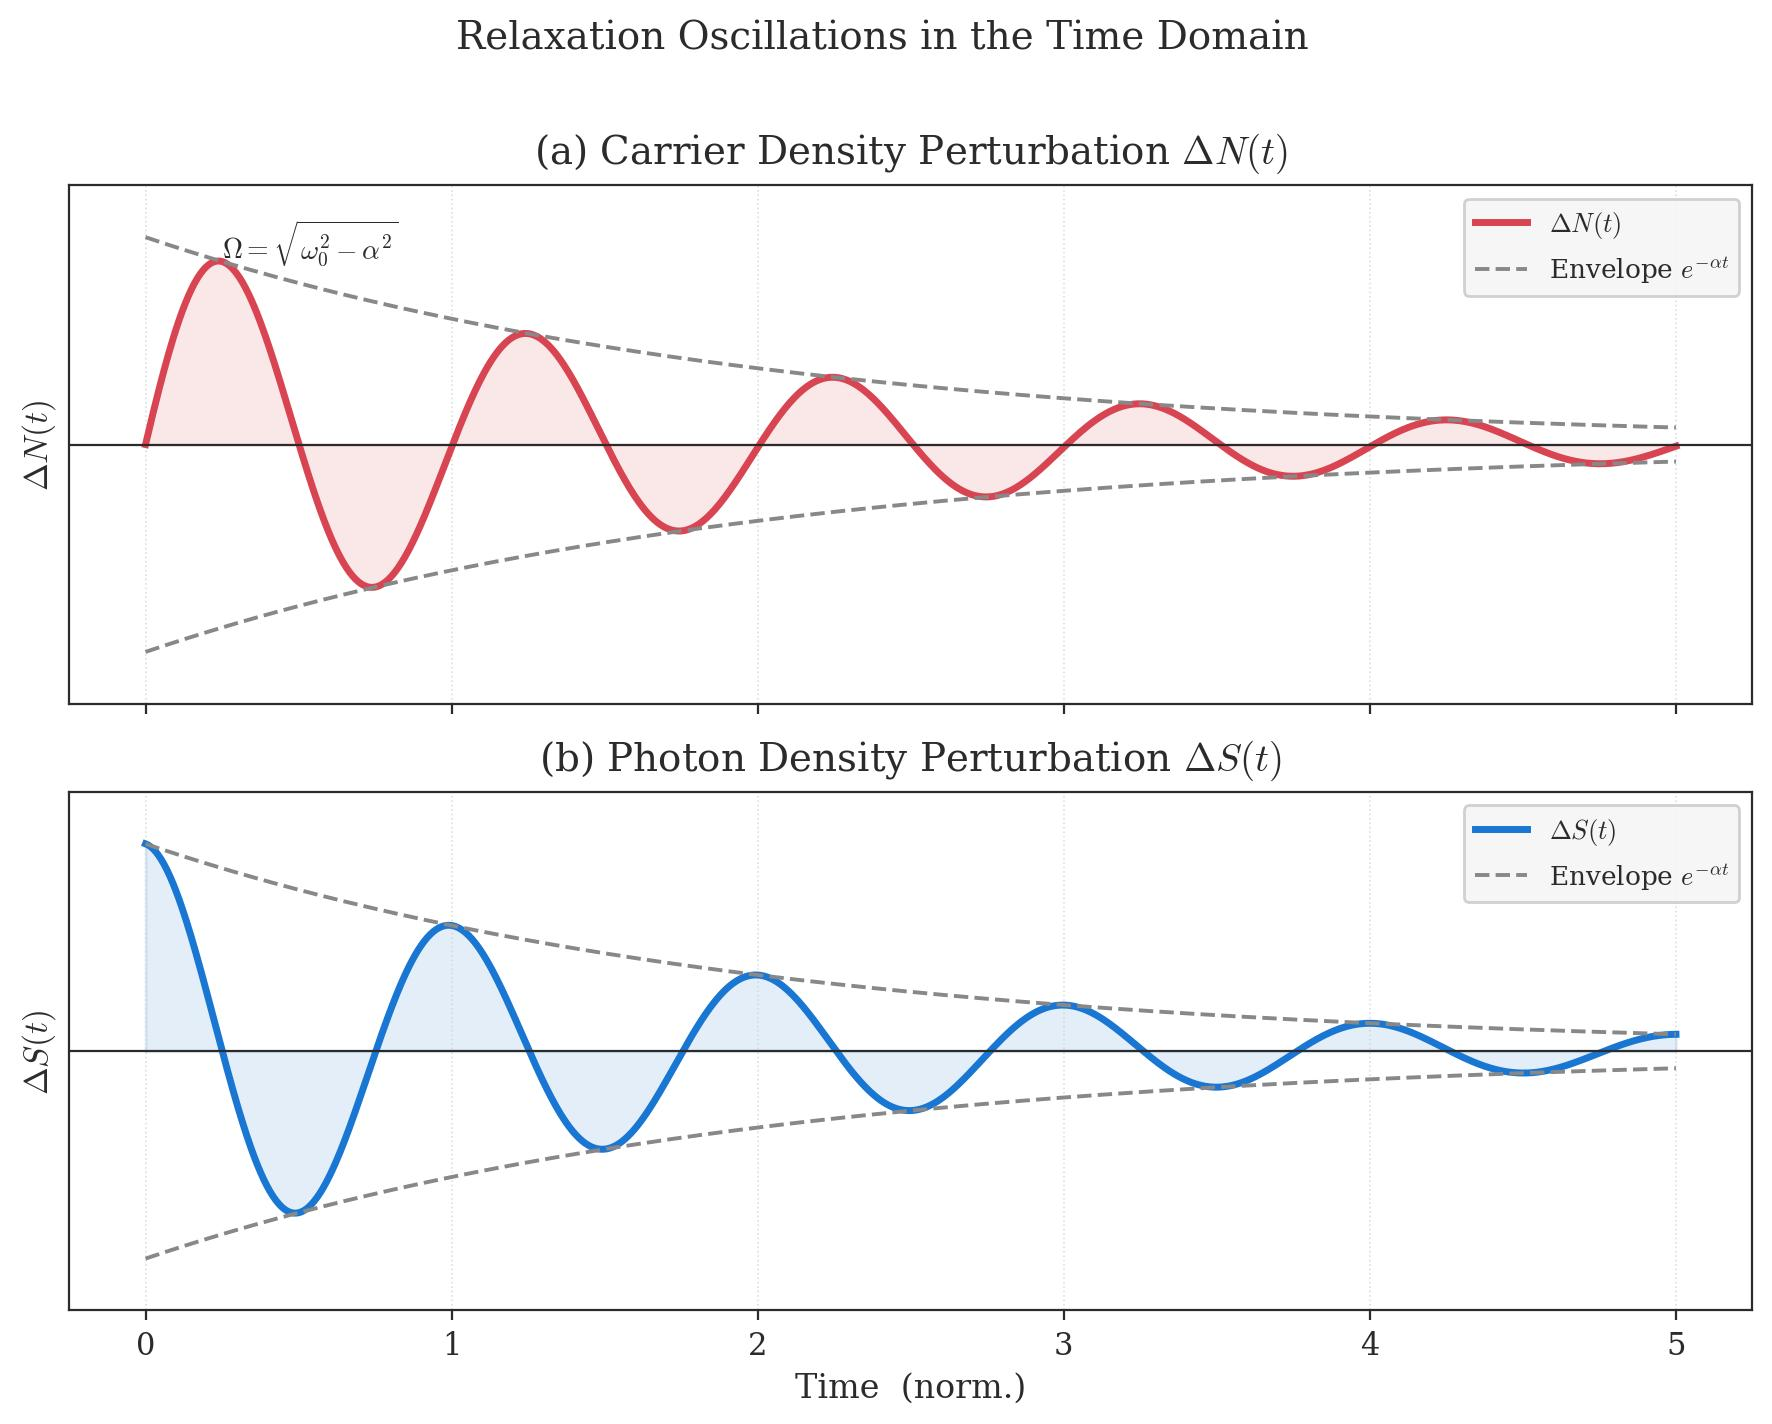
\includegraphics[width=0.7\textwidth]{Figures/Chapter 9/relaxation_oscillations.jpg}
    \caption{Relaxation Oscillations in Time Domain}
    \label{fig:relaxation_oscillations}
\end{figure}

The photon density and carrier density both oscillate at frequency $\Omega \approx \omega_r$ (for light damping), with an amplitude that decays exponentially at rate $\xi/2$. In a real laser transmitter, these ringing oscillations appear as signal distortion and inter-symbol interference if the relaxation oscillation period is comparable to the bit period. Achieving sufficient damping — by operating well above threshold — is essential for clean, pattern-independent operation.

% ------------------------------------------------------------------
\section{Single-Frequency Semiconductor Lasers}
% ------------------------------------------------------------------

\subsection{Why a Standard Fabry-Pérot Laser Is Not Single-Frequency}

An ordinary Fabry-Pérot laser diode supports multiple longitudinal modes simultaneously. In a perfectly \textbf{homogeneously broadened} gain medium (where every carrier shares the exact same transition lineshape), the first mode to reach threshold would clamp the gain globally. Once the peak gain hits the loss line, it cannot rise further, meaning all other modes would be permanently locked below threshold. The laser would perfectly oscillate in a single mode.

In reality, active atoms in the semiconductor experience slightly different local environments due to alloy fluctuations, localized strains, and thermal gradients. This leads to \textbf{inhomogeneous broadening}, where the overall gain spectrum is a superposition of many shifted individual lineshapes, forming a broad Gaussian profile:
\begin{equation*}
    \gamma(\lambda) = \gamma_o \exp\!\left(-\frac{(\lambda - \lambda_o)^2}{2\delta^2}\right)
\end{equation*}

Because the broadening is inhomogeneous, different longitudinal modes interact with different subsets of the carrier population. When the mode at $\lambda_o$ reaches threshold, it burns a "hole" in the gain spectrum at that specific wavelength (spatial hole burning), but it does \emph{not} clamp the gain at other wavelengths. This allows the gain at adjacent modes to continue rising until they too reach threshold.

The resonance condition for a Fabry-Pérot cavity of length $L$ requires the round-trip phase to be an integer multiple of $2\pi$:
\begin{equation*}
    2\beta L = 2m\pi \implies 2\left(\frac{2\pi n}{\lambda}\right) L = 2m\pi \implies m\lambda = 2nL
\end{equation*}
where $m$ is the integer mode number and $n$ is the refractive index. To find the spacing between adjacent longitudinal modes ($dm = 1$), we differentiate both sides:
\begin{equation*}
    dm \cdot \lambda + m \cdot d\lambda = 2\frac{dn}{d\lambda} d\lambda L \implies \lambda \cdot dm + \left(m - 2L\frac{dn}{d\lambda}\right) d\lambda = 0
\end{equation*}
Substituting $m = 2nL/\lambda$ and grouping terms:
\begin{equation*}
    \lambda \cdot dm + \frac{2L}{\lambda}\left(n - \lambda\frac{dn}{d\lambda}\right) d\lambda = 0
\end{equation*}
The term in the parentheses is the group index, $n_g \equiv n - \lambda\frac{dn}{d\lambda}$, which accounts for material dispersion. For adjacent modes ($dm = 1$), the magnitude of the mode spacing $d\lambda = -\Delta\lambda_f$ is:
\begin{keyresult}
    \begin{equation}
        \Delta\lambda_f = \frac{\lambda_o^2}{2 n_g L}
    \end{equation}
\end{keyresult}
If material dispersion is neglected, the group index simplifies to the refractive index ($n_g \approx n$).

The result is multimode oscillation. The total number of simultaneously oscillating modes is the spectral width over which the Gaussian gain exceeds the passive resonator loss line $\alpha_r$. By setting $\gamma(\lambda) = \alpha_r$ and solving for $\lambda$:
\begin{align*}
    \gamma_o \exp\!\left(-\frac{(\lambda - \lambda_o)^2}{2\delta^2}\right) & = \alpha_r                                                                                   \\
    -\frac{(\lambda - \lambda_o)^2}{2\delta^2}                             & = \ln\!\left(\frac{\alpha_r}{\gamma_o}\right) = -\ln\!\left(\frac{\gamma_o}{\alpha_r}\right) \\
    |\lambda - \lambda_o|                                                  & = \delta \sqrt{2 \ln\!\left(\frac{\gamma_o}{\alpha_r}\right)}
\end{align*}
This absolute deviation defines the spectral bounds of the lasing band: $\lambda_o - |\lambda - \lambda_o| \le \lambda \le \lambda_o + |\lambda - \lambda_o|$. The total lasing bandwidth is the difference between these bounds:
\begin{equation*}
    \Delta\lambda_\text{lasing} = 2|\lambda - \lambda_o| = 2\delta \sqrt{2 \ln\!\left(\frac{\gamma_o}{\alpha_r}\right)}
\end{equation*}
The total number of oscillating modes $N$ is this lasing bandwidth divided by the longitudinal mode spacing $\Delta\lambda_f$:
\begin{keyresult}
    \begin{equation}
        \text{Number of Modes } N \approx \frac{\Delta\lambda_\text{lasing}}{\Delta\lambda_f} = \frac{2\delta}{\Delta\lambda_f}\sqrt{2 \ln\!\left(\frac{\gamma_o}{\alpha_r}\right)}
    \end{equation}
\end{keyresult}

For a $300\,\mu$m long GaAs cavity with $n \approx 3.6$, the mode spacing is approximately $\Delta\lambda_f \approx 0.3\,\text{nm}$. If the gain exceeds the loss over a $15\,\text{nm}$ window, roughly $50$ modes will lase simultaneously.

Multi-mode operation is unacceptable for wavelength-division multiplexed (WDM) systems: each mode occupies a different wavelength channel, and the composite output spectrum is too broad to be routed by a wavelength-selective filter. Moreover, when the device is modulated, the mode spectrum shifts and broadens — a phenomenon called \textbf{mode partition noise} — further degrading system performance.

Shortening the cavity increases the mode spacing and can force single-mode operation, but at the cost of increased threshold current (shorter $\tau_{ph}$) and reduced output power. A better solution is to use a frequency-selective reflector.

\subsection{The Distributed Feedback (DFB) Laser}

A DFB laser etches a periodic corrugated grating directly into the waveguide along the length of the active region. The grating creates a spatially periodic variation in the effective refractive index with period $\Lambda_g$. Each corrugation reflects a tiny fraction of the propagating wave. For most wavelengths, successive reflections arrive at the next corrugation with random phase and cancel. At the Bragg wavelength, all reflections arrive in phase and add constructively, creating a strong wavelength-selective distributed reflector.

The condition for constructive interference — the Bragg condition — requires the round-trip phase per grating period to equal $2\pi$:
\begin{equation*}
    2\beta\Lambda_g = 2\pi, \qquad \beta = \frac{2\pi n_\text{eff}}{\lambda_0}
\end{equation*}

Substituting:
\begin{keyresult}
    \begin{equation}
        \lambda_B = 2\,n_\text{eff}\,\Lambda_g
    \end{equation}
\end{keyresult}

Only the longitudinal mode closest to $\lambda_B$ experiences the strong Bragg reflectivity — all others see essentially no distributed reflection and are suppressed. For a GaAs device at $\lambda_0 = 850\,\text{nm}$ with $n_\text{eff} \approx 3.5$, the required grating period is $\Lambda_g = \lambda_B/(2n_\text{eff}) \approx 120\,\text{nm}$ — achievable with electron-beam lithography.

When the injection current (and thus the carrier density) changes during modulation, the refractive index of the active region changes. Since the physical grating period $\Lambda_g$ is structurally fixed, the Bragg wavelength shifts due to changes in the effective index $n_\text{eff}$. We find this by taking the differential of the Bragg condition with respect to $n_\text{eff}$:
\begin{equation*}
    d\lambda_B = \frac{d}{d n_\text{eff}}\left(2\,n_\text{eff}\,\Lambda_g\right) dn_\text{eff} = 2\Lambda_g\,dn_\text{eff}
\end{equation*}
For a finite index perturbation $\Delta n_\text{eff}$, this shift is:
\begin{equation*}
    \Delta\lambda_B = 2\Lambda_g\,\Delta n_\text{eff}
\end{equation*}
By dividing both sides by the Bragg wavelength $\lambda_B = 2 n_\text{eff} \Lambda_g$, we obtain the fractional wavelength shift:
\begin{keyresult}
    \begin{equation}
        \frac{\Delta\lambda_B}{\lambda_B} = \frac{\Delta n_\text{eff}}{n_\text{eff}}
    \end{equation}
\end{keyresult}

This is \textbf{laser chirp}: the output wavelength shifts while the power is being modulated. In a DFB laser, the grating is inside the active region, so modulation-induced index changes directly perturb $\lambda_B$. Chirp broadens the optical spectrum during modulation and limits the dispersion-limited transmission distance in fibre.

\subsection{The Distributed Bragg Reflector (DBR) Laser}

A DBR laser separates the gain and wavelength-selection functions into physically distinct sections. The central gain section is flanked by passive grating sections that act as wavelength-selective Bragg mirrors. Current flows only through the gain section; the grating sections are passive (unbiased or separately biased).

Since the grating is outside the region where the carrier density is being modulated, changes in the drive current do not directly perturb the refractive index seen by the grating. The Bragg wavelength is therefore much more stable under modulation than in a DFB device, giving the DBR laser significantly lower chirp under direct modulation.

The trade-off is complexity: a DBR laser requires two or three separately contacted sections, demanding more careful chip design and packaging. The gain section, grating section, and (optionally) a phase-adjustment section must all be optimised and independently biased.

% ------------------------------------------------------------------
\section{From Sources to Detectors}
% ------------------------------------------------------------------

A complete optical communications link requires both a transmitter (the laser diode) and a receiver (a photodetector). Every photon generated by the laser and guided through the optical fibre must eventually be converted back into an electrical signal at the receiver. We have now fully characterised the transmitter side: from the semiconductor bandstructure, through the DH laser architecture, to the coupled rate equations governing modulation and switching. The laser emits a stream of photons that encode the data.

\begin{keyinsight}[The Completeness of the Transmitter Picture]
    The journey from a forward-biased semiconductor junction to a high-speed DFB laser diode spans five chapters. We started from isolated atomic physics (Einstein coefficients, stimulated emission), built the cavity physics (Fabry-Pérot threshold conditions, gain clamping), introduced the semiconductor material physics (bandstructure, quasi-Fermi levels, Bernard-Duraffourg), designed the device structure (DH laser, confinement factors), derived the operating characteristics (threshold current, P--I curve, slope efficiency), and finally analysed the dynamics (relaxation oscillation, modulation bandwidth, chirp).

    The next chapter shifts focus entirely to the \textbf{receiving end} of the link: how does a reverse-biased semiconductor junction convert an incoming photon stream back into an electrical current? The physics of optical absorption, quantum efficiency, responsivity, and detector noise are a mirror image of everything we have learned about emission and gain.
\end{keyinsight}

The next chapter examines the principal photodetector architectures — the PN photodiode, the PIN photodiode, and the avalanche photodiode — deriving their responsivities, speed limits, and noise characteristics from the same semiconductor physics foundation we have built throughout this sequence.
